\chapter{Структурные дефекты, возникающие при нанесении верхнего электрода}\label{ch:ch3}
\todo{Выбор платины в качестве верхнего электрода обоснован её химической инертностью, исключающей возможность окисления при контакте с HfO\(_2\)}
\section{Моделирование процесса напыления}\label{sec:ch3/sec2}
% Для бла-бла было произведено моделирование 
Для моделирования взаимодействия налетающих частиц платины с HZO были произведены квантовомеханические расчёты столкновений на основе метода Монте-Карло с помощью пакета Stopping and Range of Ions in Matter (SRIM) \cite{zieglerSRIMStoppingRange2010}. Использовалась плотность HZO, выращенного в PEALD (plasma-enhanced atomic layer deposition) процессе при температуре подложки \SI{280}{\degreeCelsius}, равная \SI{6.75}{\gram\per\cm\cubed} \cite{kimEffectProcessTemperature2022}. Оценка энергии налетаемых частиц была получена с помощью расчёта кинетической энергии атомов при лазерной абляции \cite{mutaevVLIYaNIEVERHNEYGRANICY2020}:
\todo{добавить интуиции к формулке}
\[\bar{E} = 9.92 \cdot 10^{4} A^{1/8} \tau^{1/4} Z^{3/4} (Z+1)^{3/8} (I\lambda)^{1/2}k_b,\] где \(A\) -- атомная масса распыляемого элемента, \(\tau\) -- длительность импульса, \(Z\) -- средний заряд ионов, вылетающих при абляции, \(I\) -- интенсивность лазерного излучения в \si{\watt}/\si{\cm}\(^2\), \(\lambda\) -- длина волны лазера, \(k_b\) -- постоянная Больцмана.

При импульсном лазерном напылении использовался лазер Nd:YAG с длиной волны \(\lambda=\) \SI{1064}{\nano\meter}, длительностью импульсов \(\tau=\) \SI{10}{\nano\second}. Интенсивность оценивалась как \(I=\alpha(1-\beta)\frac{J}{S}\), где \(\alpha=(1-R)^{2N}\) -- коэффициент прохождения излучения через \(N=5\) элементов оптической системы, изготовленных из кварцевого стекла с отражательной способностью \(R=0.0337\) \cite{polyanskiyRefractiveindexInfoDatabase2024} для длины волны \(\lambda\) (поглощение при этом не учитывалось), \(\beta=0.748\) -- отражательная способность платины \cite{weberHandbookOpticalMaterials2003}, \(J\) -- энергия одного импульса, \(S=\frac{\pi d^2}{4}\) -- площадь лазерного пятна с диаметром \(d\), которая была определена при проведении дополнительного эксперимента, в котором распыление платины проводилось одиночными импульсами, при этом для каждой энергии импульса формировалась дорожка из пятен (рис. \cref{fig:sem:laser_spot}). Для оценки также использовался характерный средний заряд ионов Pt при лазерном напылении $Z=0.56$ \cite[с.~141]{easonPulsedLaserDeposition2007}

\begin{figure}[ht]
    \centerfloat{
        \subcaptionbox[List-of-Figures entry]{\label{fig:sem:laser_spot:overview} Обзорный снимок, на котором видны сформированные дорожки}{%
            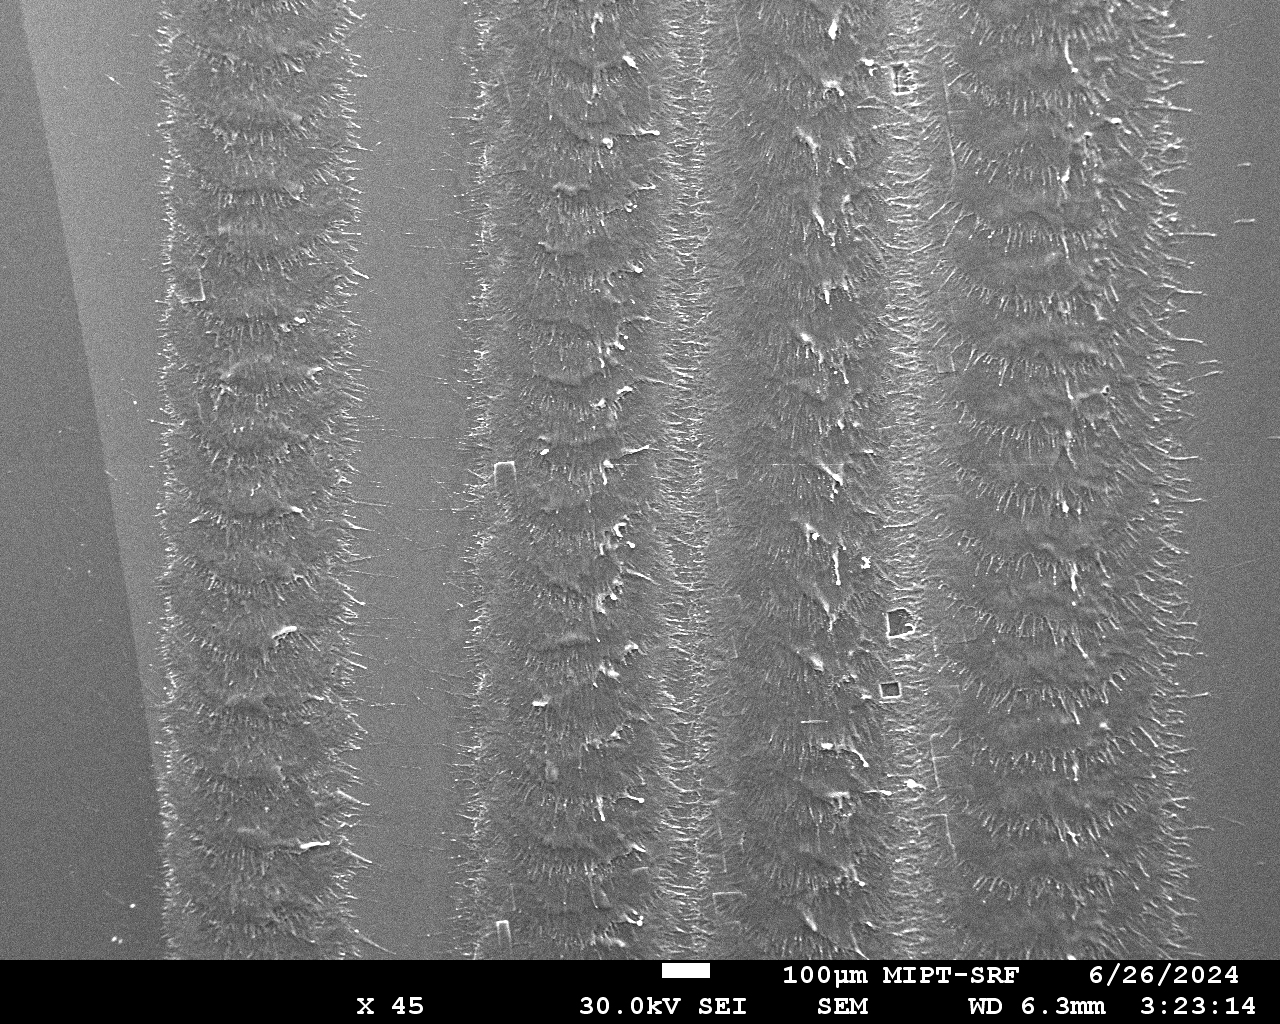
\includegraphics[width=0.45\linewidth]{sem/laser_spot/overview.jpg}}
        \subcaptionbox[List-of-Figures entry]{\label{fig:sem:laser_spot:45mJ} Энергия импульса 45 мДж}{%
            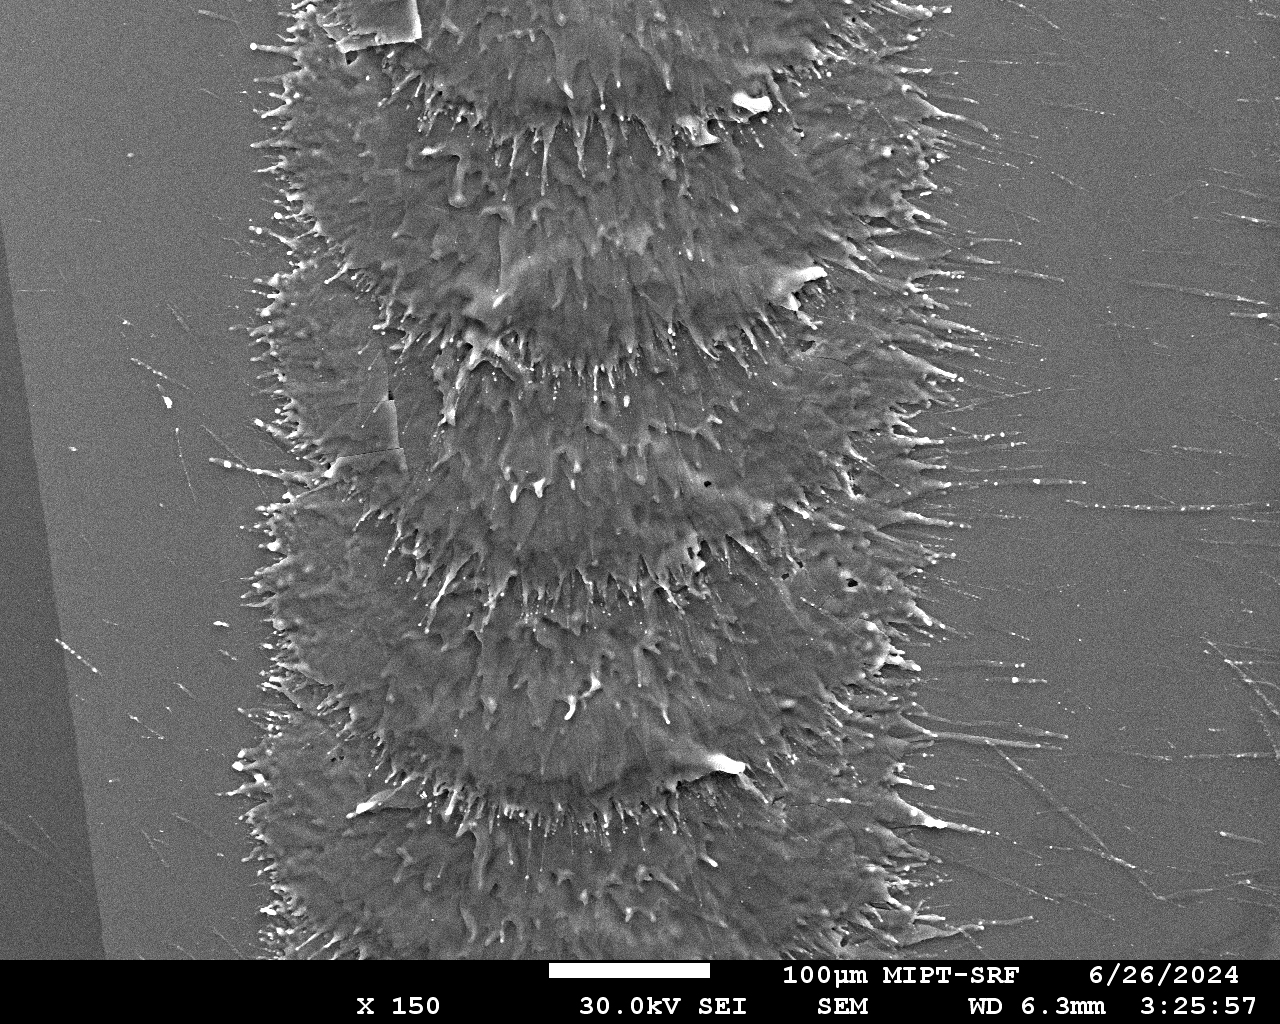
\includegraphics[width=0.45\linewidth]{sem/laser_spot/45mJ.jpg}}
        \\
        \hfill
        \subcaptionbox{\label{fig:sem:laser_spot:90mJ} Энергия импульса 93 мДж}{%
            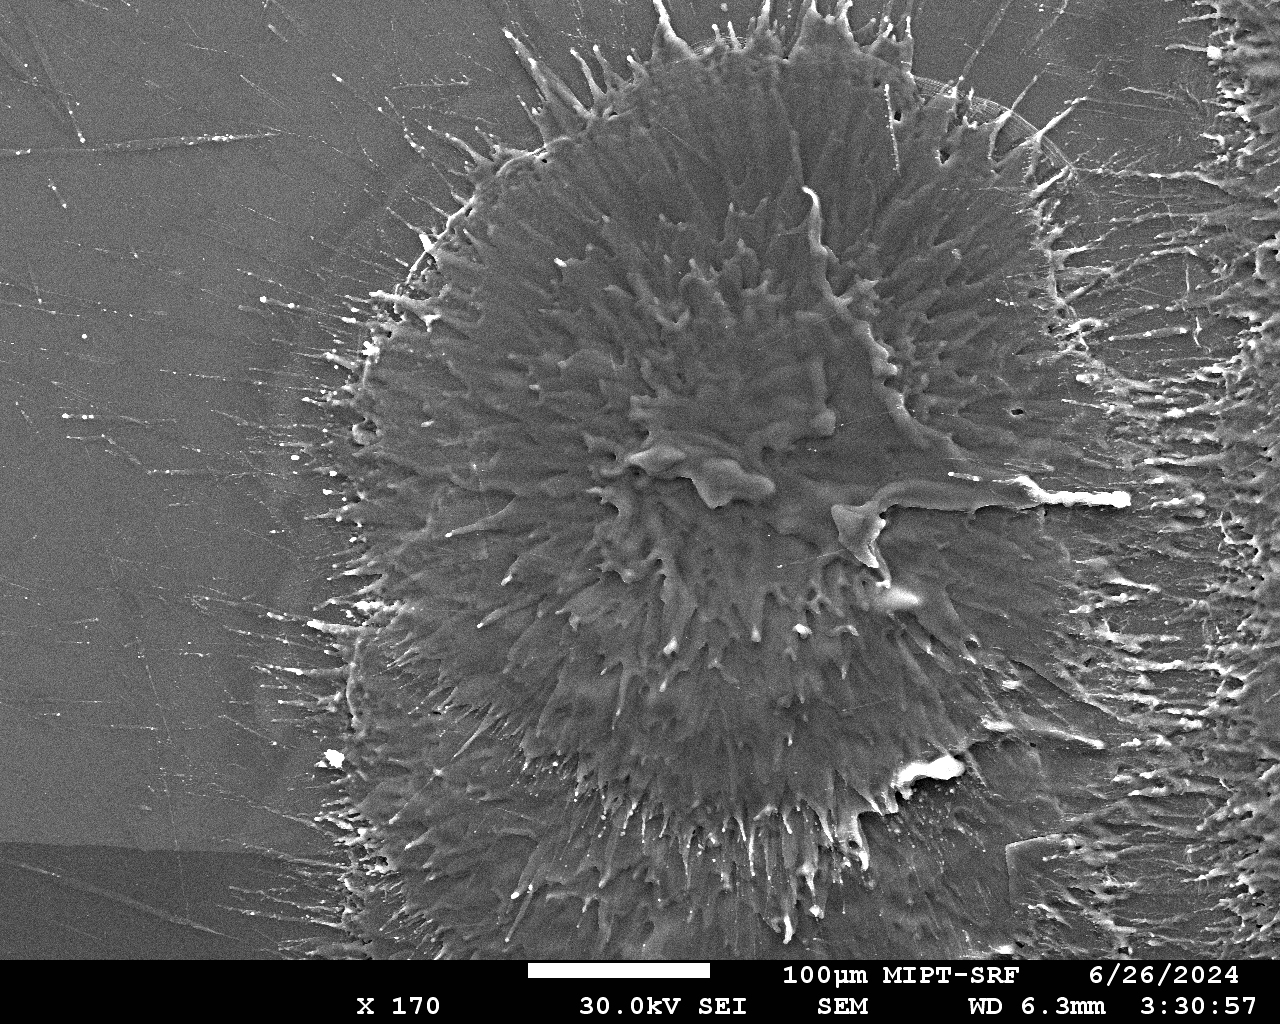
\includegraphics[width=0.45\linewidth]{sem/laser_spot/90mJ.jpg}}
        \subcaptionbox{\label{fig:sem:laser_spot:220mJ} Энергия импульса 225 мДж}{%
            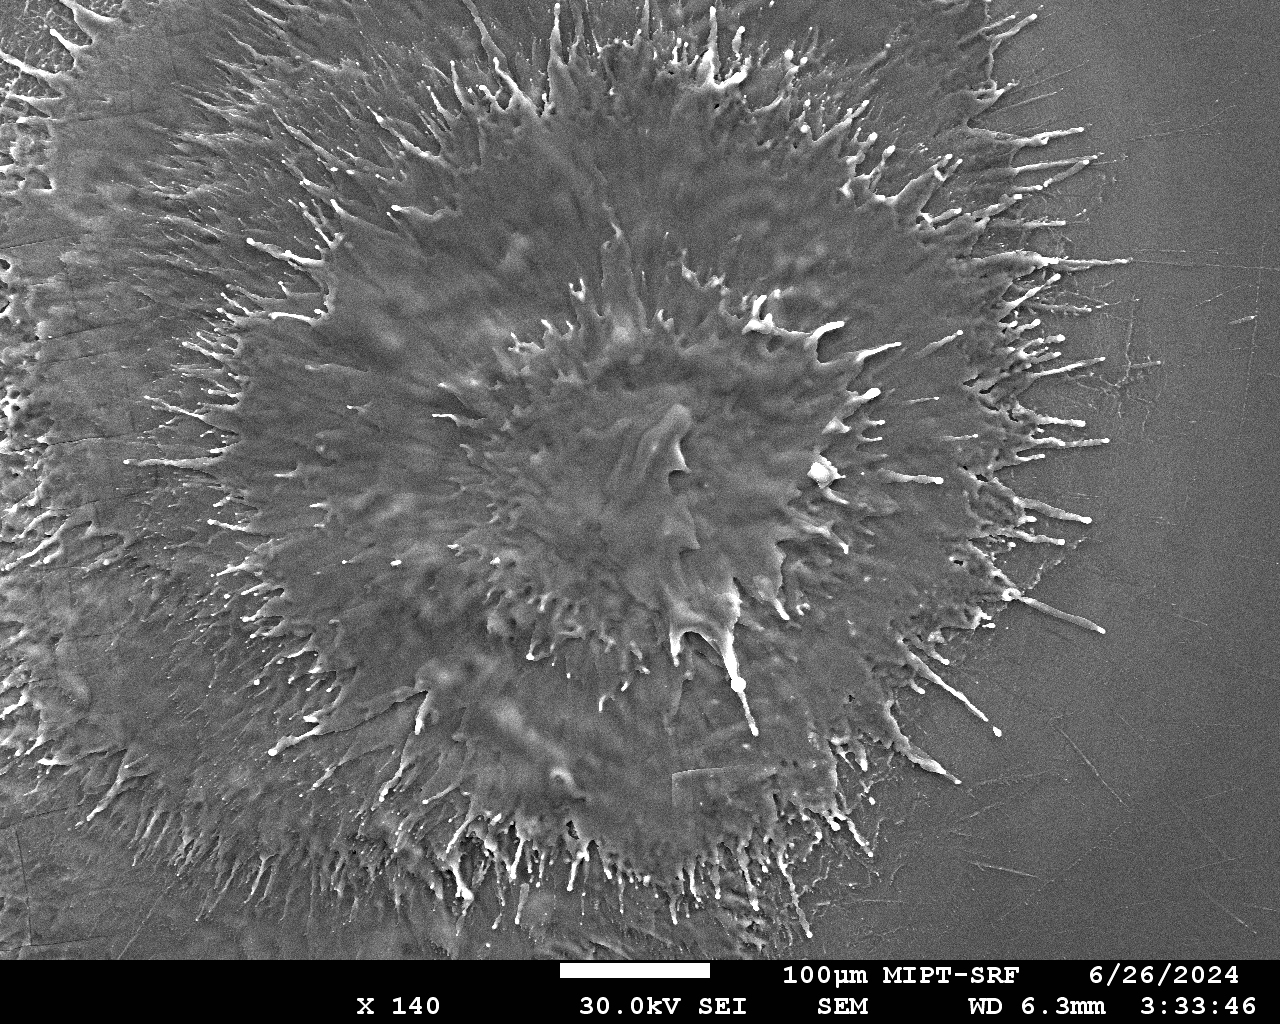
\includegraphics[width=0.45\linewidth]{sem/laser_spot/220mJ.jpg}}
    }
    \caption[Этот текст попадает в названия рисунков в списке рисунков]{Распыление платиновой мишени одиночными импульсами}\label{fig:sem:laser_spot}
\end{figure}

\begin{table} [htbp]
    \centering
    \begin{threeparttable}% выравнивание подписи по границам таблицы
        \caption{Характеристики излучения и распылённых атомов при импульсном лазерном осаждении}\label{tab:Ts0Sib}%
        \begin{tabular}{ | p{2.5cm} | p{3cm}  | p{3.5cm} | p{3cm} | p{2.3cm}l | }
            \hline
            \hline
            \centering \(J\), \si{\milli\joule} & \centering \(d\), \si{\milli\meter} & \centering \(I\), \si{\watt}/\si{\cm}\(^2\cdot 10^{8}\) & \centering \(\bar{E}\), \si{\electronvolt} & \centering \(h\), \si{\nm} & \\
            \hline
            \centering 225                      & \centering 0.52                     & \centering  18.9                                        & \centering  57                             & \centering  1.3            & \\
            \centering 145                      & \centering 0.46                     & \centering  12.2                                        & \centering  46                             & \centering 1.2             & \\
            \centering 93                       & \centering 0.41                     & \centering  7.8                                         & \centering  37                             & \centering 1.1             & \\
            \centering 45                       & \centering 0.38                     & \centering  3.8                                         & \centering  25                             & \centering 1.0             & \\
            \hline
            \hline
        \end{tabular}
    \end{threeparttable}
\end{table}

На рисунке \cref{fig:pt_distr} показано распределение атомов платины в слое HZO после 100 000 актов имплантирования. Стоит отметить, что при распылении проникновение частиц платины в HZO быстро заканчивается: расстояние между плоскостями (111) в кубической гранецентрированной решётке составляет \(\frac{a}{\sqrt{3}}\approx\) \SI{2.26}{\angstrom}, поэтому структурные свойства HZO могут измениться лишь при напылении \(\sim 4-5\) первых атомных слоёв.

\begin{figure}[ht]
    \centerfloat{
        \hfill
        \subcaptionbox[List-of-Figures entry]{\label{fig:pt_distr_151eV} \SI{151}{\electronvolt}}{%
            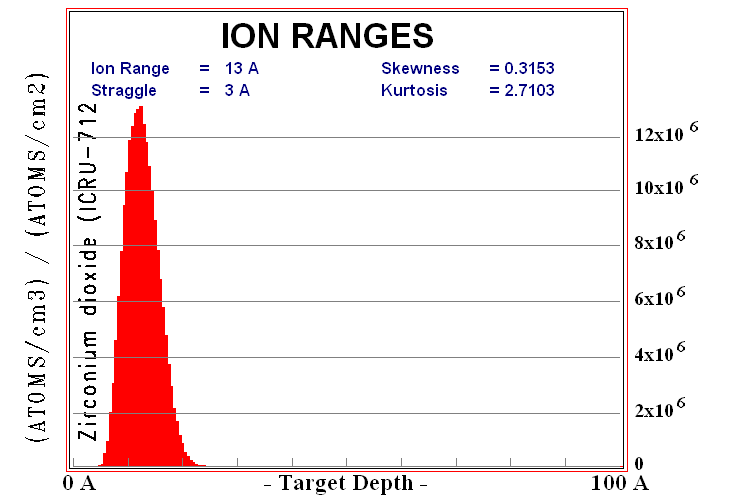
\includegraphics[width=0.5\linewidth]{srim/151 eV.png}}
        \hfill
        \subcaptionbox{\label{fig:pt_distr_121eV}\SI{121}{\electronvolt}}{%
            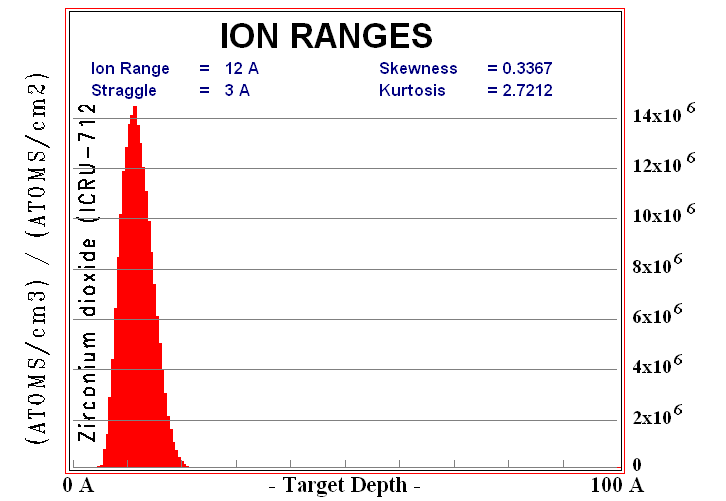
\includegraphics[width=0.5\linewidth]{srim/121 eV.png}}
        \hfill
        \\
        \subcaptionbox{\label{fig:pt_distr_97eV}\SI{97}{\electronvolt}}{%
            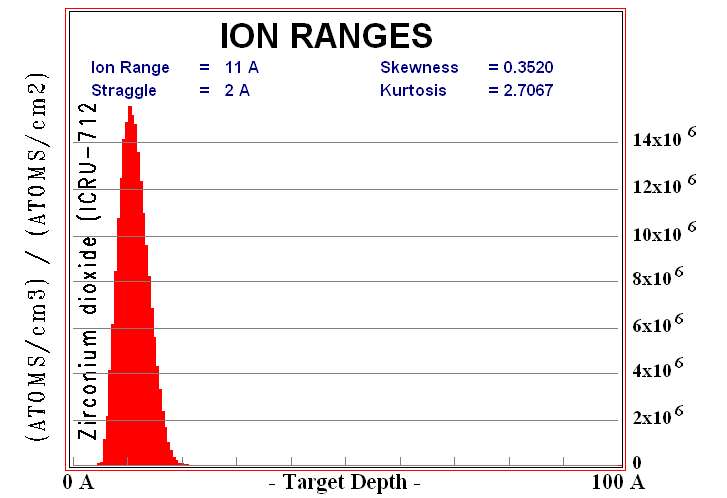
\includegraphics[width=0.5\linewidth]{srim/97 eV.png}}
        \hfill
        \subcaptionbox{\label{fig:pt_distr_68eV}\SI{68}{\electronvolt}}{%
            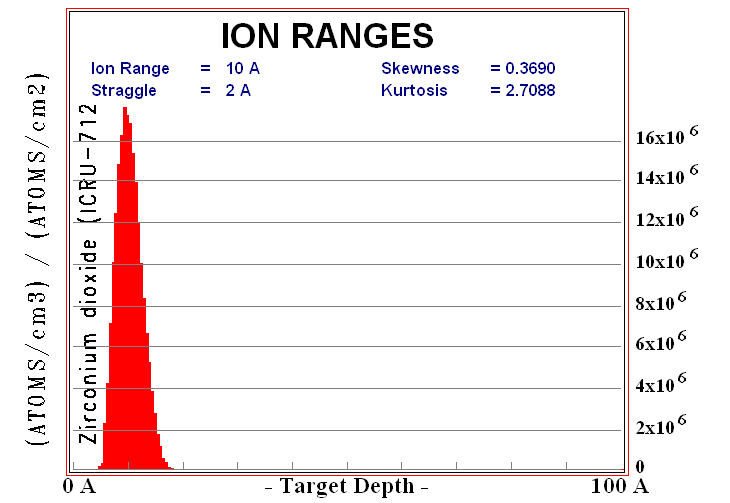
\includegraphics[width=0.5\linewidth]{srim/68 eV.png}}
        \hfill
    }
    \caption[Этот текст попадает в названия рисунков в списке рисунков]{Распределение атомов платины в плёнке HZO после 100 000 актов распыления при различных энергиях распыляемых частиц}\label{fig:pt_distr}
\end{figure}


% \section{Встроенные поля}

% Различная концентрация кислородных вакансий в плёнке HZO до циклирования приводит к образованию встроенных (built-in) электрических полей \(E_\text{bi}\) \cite{pesicImpactChargeTrapping2016} и пиннингу доменов\todo{ref}. При приложении внешнего электрического поля \(E_\text{ext}\), эффективное поле \(E_\text{eff}\) в СЭ слое складывается из суммы полей: \(\boldsymbol{E_\text{eff}} = \boldsymbol{E_\text{bi}} + \boldsymbol{E_\text{ext}}\). Таким образом, приводя к сдвигу и асимметрии ВАХ относительно нулевого напряжения. В случае наличия противоположно направленных встроенных полей в образце, происходит расщепление пиков переполяризационного тока на вольт-амперных характеристиках \cite{schenkElectricFieldCycling2014}.

% Встроенные поля приводят к расщеплению пиков переполяризационного тока на вольт-амперных характеристиках (ВАХ) за счёт

% Одной из причиной образования внутренних полей является наличие градиента механических напряжений (флексоэлектрический эффект)

\section{Флексоэлектрический эффект}\label{sec:ch3/flexoelectric}

Флексоэлектрическим эффектом называется возникновение поляризации в диэлектрике при его изгибе. Электрическое поле, созданное за счёт наличия градиента механических напряжений, может быть оценено по формуле \cite{gruvermanMechanicalStressEffect2003}

\[E_\text{eff}=\frac{f}{\varepsilon\varepsilon_0}\frac{\partial u}{\partial z} = \frac{e}{4\pi\varepsilon_0 a}\frac{\partial u}{\partial z},\]
где \(f\) -- флексоэлектрический коэффициент, \(\epsilon\) -- диэлектрическая проницаемость, \(\epsilon_0\) -- диэлектрическая постоянная, \(\frac{\partial u}{\partial z}\) -- градиент механических напряжений, \(e\) -- заряд электрона, \(a\) -- постоянная решётки.

Градиент концентрации частиц платины в плёнке HZO \(\frac{\partial n}{\partial z}\) вызывает градиент механических напряжений \(\frac{\partial u}{\partial z}\approx\frac{u_{max}}{\Delta z}\), где \(u_\text{max}\) -- максимальное механическое напряжение, возникающее на глубине с максимальной концентрацией частиц платины, а \(\Delta z\) -- ширина распределения.

Таким образом, выдвинув предположение о флексоэлектрической природе встроенных полей \(E_\text{bi}\) и определив их величину по результатам электрофизических измерений (рис. \cref{fig:probe_station:pq}) можно получить оценку для величины механических напряжений в плёнке HZO, вызванных имплантированными частицами платины:
\[u_\text{max}= E_{bi}\frac{4\pi\varepsilon_0 a}{e}\Delta z\]

Полученные значения механических напряжений (табл. \ref{tab:stress}) имеют характерные величины, соответствующие экспериментальным значениям, при которых были получены сегнетоэлектрические свойства в оксиде-гафния\todo{процитировать что-нибудь, мб ga-doped поискать напряжения, либо ещё в какой-то статье было (в PZT PFM Были вроде, но всё таки HfO2 поискать)}.


\begin{table} [htbp]
    \centering
    \begin{threeparttable}% выравнивание подписи по границам таблицы
        \caption{Механические напряжения}\label{tab:stress}%
        \begin{tabular}{ | p{2.5cm} | p{2.5cm} | p{2.5cm} | p{2.5cm}  | p{3cm}l | }
            \hline
            \hline
            \centering \(\bar{E}\), \si{\electronvolt} & \centering \(E_{bi}\), \si{\volt} & \centering \(\sigma\), \si{\angstrom} & \centering \(u_\text{max}\), \% & \centering \(\frac{\partial u}{\partial z}\), \si{\meter}\(^{-1}\cdot 10^7\) & \\
            \hline
            \centering 151                             & \centering 1.5                    & \centering  3                         & \centering  0.51                & \centering 3.4                                                               & \\
            \centering 121                             & \centering1.7                     & \centering  3                         & \centering  0.58                & \centering 3.9                                                               & \\
            \centering 97                              & \centering 2.0                    & \centering  2                         & \centering  0.45                & \centering 4.5                                                               & \\
            \centering 68                              & \centering 2.3                    & \centering  2                         & \centering  0.52                & \centering 5.2                                                               & \\
            \hline
            \hline
        \end{tabular}
    \end{threeparttable}
\end{table}

% \nomenclature{АСО}{атомно-слоевое осаждение}
% \nomenclature{PUND}{positive up negative down, электрофизический метод измерения остаточной поляризации}

\FloatBarrier
